This chapter explains how the VietFlood prototype was built after the design decisions in the previous chapter. The discussion follows the same implementation order as the report format: development tools, service communication, authentication, report processing, shared backend utilities, real-time tracking, mobile features, web dashboard features, deployment, and user management.

The implementation is divided across four repositories: the NestJS backend, the mobile application, the web dashboard, and the shared common package. The backend provides the API gateway, authentication service, reports service, message queues, cache access, media handling, and live tracking gateway. The mobile application supports citizen reporting and relief viewing. The web dashboard supports administrator review and report status control. The shared package keeps repeated infrastructure code in one place so the services can stay focused on their own responsibilities.

\newcommand{\vfplaceholderfigure}[5]{%
\begin{figure}[H]
    \centering
    \IfFileExists{images/#1}{%
        \includegraphics[width=#2\linewidth,height=#3\textheight,keepaspectratio]{images/#1}%
    }{%
        \fbox{%
            \begin{minipage}[c][#3\textheight][c]{#2\linewidth}
                \centering
                Placeholder for VietFlood figure\\[0.3cm]
                Suggested content: #4\\[0.25cm]
                File name:\\[0.1cm]
                \resizebox{0.9\linewidth}{!}{\texttt{\detokenize{#1}}}
            \end{minipage}
        }%
    }%
    \caption{#4}
    \label{#5}
\end{figure}
}

\section{Technique and Tools}

VietFlood was implemented as a multi-platform system rather than as a single application. The backend was written with NestJS and TypeScript \cite{nestjsDocs,typescriptDocs}. The mobile client was built with Expo React Native \cite{expoDocs,reactNativeDocs}. The administrator dashboard was developed with Next.js \cite{nextjsDocs}. These tools were selected because they allow one TypeScript-based workflow to cover server code, mobile screens, and web dashboard components while still leaving each platform with its own deployment target.

\vspace{1em}
\noindent
\textbf{a) Version Control and Build Tools:}

The source code is managed with Git. The backend is arranged as a NestJS workspace containing the API gateway, authentication service, and reports service. Each backend application has a Dockerfile, and Docker Compose starts the backend services together with RabbitMQ and Redis for local development \cite{dockerComposeDocs}. For deployment, the workflow builds Docker images for the gateway, auth service, and reports service before running them on Azure App Service \cite{azureAppServiceContainersDocs}.

\vspace{1em}
\noindent
\textbf{b) Front-end Development:}

The mobile app uses Expo, React Native, and TypeScript \cite{expoDocs,reactNativeDocs,typescriptDocs}. React Navigation controls movement between authentication, citizen, relief, report, and profile screens. Redux Toolkit stores authentication state \cite{reduxToolkitDocs}. Expo SecureStore is used when the user chooses to keep the login after closing the app. Device location and image picker APIs support flood report creation because a report usually needs both a place and visible evidence.

The web dashboard uses Next.js, React, TypeScript, and Tailwind CSS \cite{nextjsDocs,reactDocs,typescriptDocs,tailwindDocs}. Its main audience is the administrator. The dashboard loads reports from the backend, formats report status values, displays evidence thumbnails, filters reports, and sends status changes through the API gateway.

\vspace{1em}
\noindent
\textbf{c) Back-end Development:}

The backend follows a microservices style using NestJS microservice support \cite{nestjsMicroservicesDocs}. The API gateway exposes REST endpoints and the Socket.IO gateway \cite{socketioDocs}. The auth service owns registration, login, profile loading, profile updates, refresh tokens, logout, and user administration. The reports service owns report creation, report retrieval, report update, report deletion, evidence metadata, and cache refresh logic.

RabbitMQ carries messages from the gateway to the backend services \cite{rabbitmqConfirmsDocs}. Authentication requests are sent to the auth queue, while report requests are sent to the reports queue. The gateway adds timeout and retry behavior so client requests can fail in a controlled way when a service is unavailable.

\vspace{1em}
\noindent
\textbf{d) Database and Media Storage:}

PostgreSQL is used for durable data: users, refresh tokens, and reports. TypeORM maps these tables into service entities \cite{typeormDocs}. Redis stores selected report cache entries so repeated report lookups do not always need to read from PostgreSQL \cite{redisDocs}. Cloudinary stores report evidence files \cite{cloudinaryUploadDocs}. The database keeps only the media metadata, such as public URL, public ID, and resource type, using JSONB fields where the report needs flexible evidence data \cite{postgresqlJsonDocs}.

\vspace{1em}
\noindent
\textbf{e) Cloud Service and Runtime Configuration:}

The deployed backend uses Azure App Service as its runtime target. Sensitive values are not written directly into the source code. They are passed through environment variables, including database URL, Redis settings, RabbitMQ credentials, JWT secrets, refresh-token secret, Cloudinary credentials, and administrator seed values. This separation lets the same codebase run locally and in the deployed environment with different configuration values.

\begin{table}[H]
    \centering
    \caption{Main implementation tools used in VietFlood.}
    \setlength{\tabcolsep}{10pt}
    \renewcommand{\arraystretch}{1.35}
    \begin{tabular}{|p{3.4cm}|p{9.2cm}|}
        \hline
        \textbf{Area} & \textbf{Tools and implementation use} \\
        \hline
        Backend & NestJS, TypeScript, TypeORM, RabbitMQ, Socket.IO, JWT, bcrypt, and Docker. \\
        \hline
        Shared library & \texttt{vietflood\_common} for logging, Redis access, and Cloudinary operations. \\
        \hline
        Database and cache & PostgreSQL for stored records and Redis for report cache entries. \\
        \hline
        Media storage & Cloudinary for uploaded report evidence and generated media URLs. \\
        \hline
        Mobile app & Expo, React Native, React Navigation, Redux Toolkit, SecureStore, image picker, and device location. \\
        \hline
        Web dashboard & Next.js, React, TypeScript, Tailwind CSS, token storage, and admin report review. \\
        \hline
        Deployment & Docker Compose, Docker Hub, GitHub Actions, and Azure App Service. \\
        \hline
    \end{tabular}
    \label{tab:vietflood-implementation-tools}
\end{table}

\section{Messaging Broker Implementation}

RabbitMQ is used as the communication layer between the public API gateway and the internal backend services \cite{rabbitmqConfirmsDocs,nestjsMicroservicesDocs}. The gateway receives HTTP requests from mobile and web clients, prepares the request payload, and sends it to the service that owns the business logic. The auth service listens on \texttt{auth\_queue}. The reports service listens on \texttt{reports\_queue}.

The gateway does not directly import report or authentication logic. Instead, it sends message patterns such as \texttt{register}, \texttt{sign\_in}, \texttt{profile}, \texttt{refresh}, \texttt{logout}, \texttt{create}, \texttt{get\_all\_by\_users}, \texttt{update}, and \texttt{delete}. This keeps the gateway as a transport boundary and keeps each service responsible for its own data rules.

Gateway calls are wrapped with timeouts and retries. Upload-heavy requests, such as report creation and report update, are allowed more time because they may involve Cloudinary. Smaller queries use shorter limits. When a backend service returns an error or cannot respond, the gateway turns that failure into a controlled HTTP response instead of leaving the mobile or web client waiting.

\begin{table}[H]
    \centering
    \caption{Comparison of message brokers for the VietFlood backend.}
    \setlength{\tabcolsep}{8pt}
    \renewcommand{\arraystretch}{1.45}
    \begin{tabular}{|p{3.1cm}|p{3.2cm}|p{3.2cm}|p{3.2cm}|}
        \hline
        \textbf{Criteria} & \textbf{RabbitMQ} & \textbf{Redis Pub/Sub} & \textbf{Kafka} \\
        \hline
        Request-response work & Suitable for gateway commands, queues, and acknowledgements. & Fast, but weaker for durable command handling. & Powerful, but too heavy for this prototype. \\
        \hline
        Operational cost & Simple to run locally with two backend services. & Simple, but already used for cache in VietFlood. & Requires more setup and topic management. \\
        \hline
        VietFlood usage & Used for auth and report service communication. & Used separately as the report cache layer. & Not used in the current system. \\
        \hline
    \end{tabular}
    \label{tab:vietflood-broker-comparison}
\end{table}

\vfplaceholderfigure
    {figure4-1-rabbitmq-communication-flow.png}
    {0.76}
    {0.36}
    {RabbitMQ communication flow between the API gateway, auth service, reports service, auth queue, and reports queue.}
    {fig:vietflood-rabbitmq-flow}

\section{Authentication and Authorization Implementation}

VietFlood uses username-password authentication with short-lived access tokens and refresh tokens. User passwords are hashed with bcrypt before they are stored \cite{provos1999bcrypt}. After a successful login, the auth service signs an access token and creates a refresh token. The access token follows the JSON Web Token format \cite{jones2015jwt}. Its payload carries the user ID, username, role, first name, and last name, which allows the gateway to apply role checks on protected routes.

\subsection{Authentication Mechanism Implementation}

\textbf{a) Registration Process}

Registration is handled by the auth service. Before creating a user, the service checks whether the submitted email, username, or phone number is already used. If any of these values already exists, the request is rejected. If the values are available, the password is hashed using bcrypt with ten salt rounds, and the new record is saved in the \texttt{users} table.

The mobile registration screen sends the fields required by the user entity, including email, username, password, phone number, name fields, date of birth, and address information. The backend returns a small success response after creation. It does not send the stored password hash or the full database record back to the client.

\begin{figure}[H]
    \centering
    \begin{minipage}[b]{0.48\linewidth}
        \centering
        \IfFileExists{images/figure4-2-mobile-registration.jpg}{%
            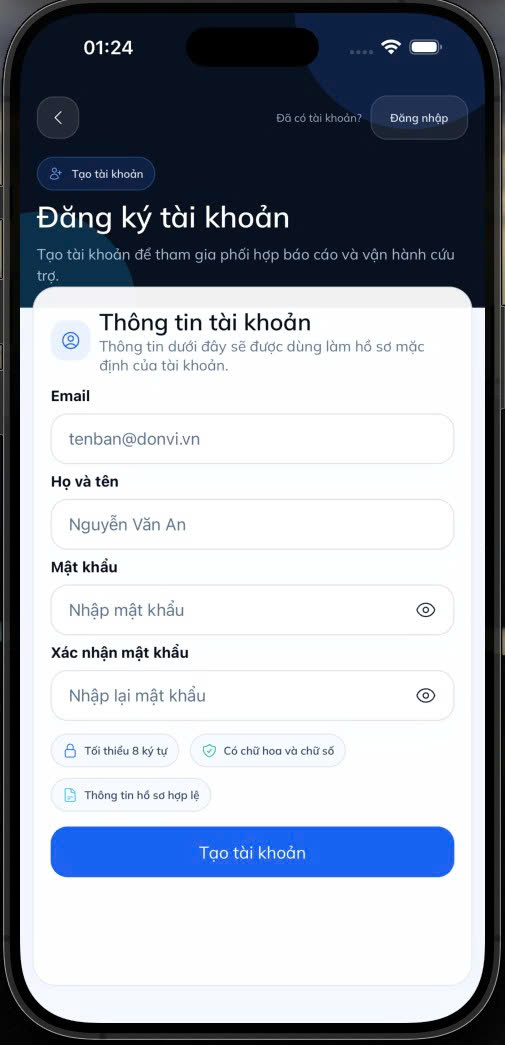
\includegraphics[width=\linewidth,height=0.36\textheight,keepaspectratio]{images/figure4-2-mobile-registration.jpg}%
        }{%
            \fbox{\begin{minipage}[c][5.2cm][c]{0.92\linewidth}\centering Placeholder\\[0.2cm]\resizebox{0.9\linewidth}{!}{\texttt{figure4-2-mobile-registration.jpg}}\\[0.2cm]Mobile registration screen\end{minipage}}%
        }
        \caption{Citizen registration screen in the VietFlood mobile app.}
        \label{fig:vietflood-mobile-registration}
    \end{minipage}
    \hfill
    \begin{minipage}[b]{0.48\linewidth}
        \centering
        \IfFileExists{images/figure4-3-mobile-login.jpg}{%
            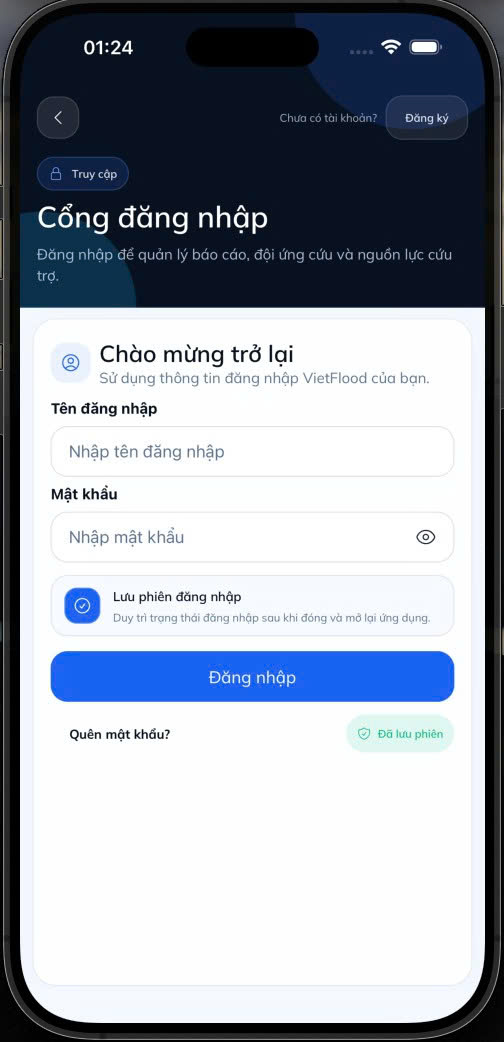
\includegraphics[width=\linewidth,height=0.36\textheight,keepaspectratio]{images/figure4-3-mobile-login.jpg}%
        }{%
            \fbox{\begin{minipage}[c][5.2cm][c]{0.92\linewidth}\centering Placeholder\\[0.2cm]\resizebox{0.9\linewidth}{!}{\texttt{figure4-3-mobile-login.jpg}}\\[0.2cm]Mobile login screen\end{minipage}}%
        }
        \caption{Citizen login screen in the VietFlood mobile app.}
        \label{fig:vietflood-mobile-login}
    \end{minipage}
\end{figure}

\textbf{b) Login Process}

Login is exposed through the \texttt{/auth/sign\_in} endpoint. The auth service searches for the user by username, compares the submitted password with the stored bcrypt hash, and rejects invalid credentials. If the credentials are valid, the service returns an access token and a refresh token.

The mobile app and web dashboard use the login response in different ways. On mobile, the user can choose between a saved login and a session-only login. A saved login writes tokens to SecureStore, while a session-only login keeps them in memory. On the web dashboard, tokens are stored in browser storage, and the dashboard loads the current profile before showing admin-only pages. If the loaded profile is not an administrator profile, the dashboard does not allow entry.

\vfplaceholderfigure
    {figure4-4-web-admin-login.jpg}
    {0.72}
    {0.36}
    {Admin login page in the VietFlood web dashboard.}
    {fig:vietflood-web-login}

\subsection{Refresh Token Implementation}

Refresh tokens are stored as hashed values in the \texttt{refresh\_tokens} table. Each row is connected to one user and includes expiration and revocation information. When a user signs in again, the refresh-token service can update the existing row instead of creating an unlimited number of active tokens for the same account.

The refresh endpoint lets the mobile app and web dashboard request a new access token without asking the user to log in again. On mobile, the token storage helper keeps the same storage behavior that was selected at login time. A session-only login remains session-only after refresh, while a saved login writes the refreshed values back to SecureStore.

\vfplaceholderfigure
    {figure4-6-token-refresh-flow.png}
    {0.76}
    {0.34}
    {Refresh-token flow from mobile or web client through the API gateway, auth service, refresh-token table, and new access token response.}
    {fig:vietflood-refresh-token-flow}

\subsection{Authorization Process Implementation}

Authorization is checked at the API gateway. JWT guards validate the token, and role guards decide whether the route can be used by a citizen, relief user, or administrator. Citizens can create reports and manage their own submitted reports. Relief users can read reports and inspect report locations for response work. Administrators can review evidence, update report status, and manage users.

This permission split is important in VietFlood. Relief users are not responsible for verifying or rejecting reports in the current system. Their screens support field awareness, such as report lists, report details, and map views. Verification, rejection, and resolution remain administrator actions.

\section{Report Processing and Evidence Upload Implementation}

Report creation begins in the mobile application. The citizen fills in category, description, address, coordinates, urgency, severity, and optional evidence images. The app sends this data as multipart form data so text fields and image files can travel in the same request.

The API gateway receives the files in memory and uploads them to Cloudinary under the report evidence folder \cite{cloudinaryUploadDocs}. It then sends the cleaned report payload and evidence metadata to the reports service through RabbitMQ. The reports service stores the report in PostgreSQL. Category values are kept as arrays, and evidence is stored as JSONB values containing the public URL, public ID, and resource type \cite{postgresqlJsonDocs}. After saving, the service writes a Redis cache entry for the report ID \cite{redisDocs}.

\vfplaceholderfigure
    {figure4-7-report-processing-flow.png}
    {0.82}
    {0.38}
    {Report creation flow from mobile form submission to Cloudinary upload, RabbitMQ message, PostgreSQL insert, and Redis cache write.}
    {fig:vietflood-report-processing-flow}

\subsection{Report Update and Delete Implementation}

Report update reuses the same upload path as report creation. If the citizen attaches new evidence, the gateway uploads the files to Cloudinary and adds the returned metadata to the update payload. The reports service checks that the report belongs to the user, merges new evidence with the old evidence, updates image URLs, removes the outdated Redis cache entry, and writes a fresh cache entry.

Report deletion also checks ownership before changing data. The reports service reads Cloudinary public IDs from the stored evidence metadata and calls the shared bulk-delete helper when media exists. It then deletes the report row from PostgreSQL and removes the related Redis cache key.

\section{Public Library Implementation}

The shared backend package is implemented as \texttt{vietflood\_common}. It contains reusable infrastructure services for logging, Redis, and Cloudinary. Without this package, the gateway, auth service, and reports service would need to repeat the same connection and helper logic.

The Cloudinary helper supports buffer upload, file-path upload, base64 upload, single delete, bulk delete, rename, optimized image URL generation, and raw URL generation. In the report workflow, the gateway uses buffer upload for evidence files, while the reports service uses bulk delete when a report is removed.

The Redis helper wraps common operations such as \texttt{set}, \texttt{get}, \texttt{del}, and \texttt{publish} \cite{redisDocs}. VietFlood mainly uses it for report cache records. The logger service adds service names and request context to logs, which makes backend behavior easier to trace while running several services at the same time.

\vfplaceholderfigure
    {figure4-8-common-library-structure.png}
    {0.76}
    {0.34}
    {Shared common library structure showing LoggerService, RedisService, CloudinaryService, and the backend modules that import them.}
    {fig:vietflood-common-library}

\section{Real-Time Tracking Implementation}

VietFlood includes a Socket.IO gateway for live location sharing \cite{socketioDocs}. The client sends a location event with latitude, longitude, accuracy, heading, speed, and timestamp. The gateway validates the latitude and longitude before broadcasting. Invalid coordinates return a location error to the sender, while valid coordinates are sent to connected clients.

The gateway also handles socket connection and disconnection events. When a client disconnects, other connected clients can be informed that the user is no longer available. This feature supports response-oriented scenarios because a relief screen can receive a citizen's latest location while the report is being handled. In the current prototype, the implementation proves the live communication path; authenticated sockets and stored location history can be added later.

\vfplaceholderfigure
    {figure4-9-live-tracking-flow.png}
    {0.76}
    {0.34}
    {Socket.IO live tracking flow with send-location, receive-location, location-error, and user-disconnected events.}
    {fig:vietflood-live-tracking-flow}

\section{Mobile Citizen Feature Implementation}

\subsection{Report List and Profile Access}

The mobile app provides the main citizen workflow after login. It loads the user profile through an authenticated endpoint and retrieves reports through the report service wrapper. The wrapper normalizes backend data before rendering because some fields may appear in different naming styles across the backend and client models.

The citizen report list displays submitted reports with status, category, location, and evidence information. Status labels are normalized before display so the interface remains stable when the backend returns older or alternate status values. This makes the report list more tolerant while the prototype is still evolving.

\vfplaceholderfigure
    {figure4-10-mobile-report-list.jpg}
    {0.72}
    {0.36}
    {Citizen report list or citizen home screen showing submitted reports, status labels, and report location information.}
    {fig:vietflood-mobile-report-list}

\subsection{Create Report Implementation}

The create-report screen collects the information needed for a useful flood report: category, description, address, latitude, longitude, urgency, severity, and evidence images. Province and ward selection uses data from the Vietnam Provinces Open API \cite{vietnamProvincesOpenApi}. If the user grants location permission, the mobile app can fill coordinate values from the device. The final request is sent as multipart form data so the backend receives both report fields and files.

\vfplaceholderfigure
    {figure4-11-mobile-create-report.jpg}
    {0.72}
    {0.36}
    {Create report form in the VietFlood mobile app.}
    {fig:vietflood-mobile-create-report}

\vfplaceholderfigure
    {figure4-12-mobile-evidence-upload.jpg}
    {0.72}
    {0.36}
    {Evidence upload in the VietFlood mobile app.}
    {fig:vietflood-mobile-evidence-upload}

\section{Relief Feature Implementation}

The relief side of the mobile app is built for reading and locating flood reports. The relief report list shows submitted cases, and the detail view presents description, category, address, evidence, and current status. The map screen helps response users understand where reports are placed geographically.

The relief role is deliberately narrower than the administrator role. Relief users can use report and map information for response coordination, but they do not verify, reject, or resolve reports. The mobile app follows this rule by focusing relief screens on viewing, navigation, and situational awareness.

\vfplaceholderfigure
    {figure4-13-relief-report-list.jpg}
    {0.72}
    {0.36}
    {Relief report list in the mobile app.}
    {fig:vietflood-relief-report-list}

\vfplaceholderfigure
    {figure4-14-relief-map.jpg}
    {0.72}
    {0.36}
    {Relief map screen in the mobile app.}
    {fig:vietflood-relief-map}

\section{Web Dashboard Implementation}

The web dashboard is the administrator workspace. It starts from an admin login screen, stores the returned tokens, and loads the current profile before displaying protected pages. The reports overview loads report records from the backend, formats dates for Vietnamese display, translates category and status values, extracts thumbnail images from evidence, and shows reporter information when it is available.

The dashboard includes search and status filtering. Search can match reporter name, account name, phone number, location, and description. Status filtering supports pending, verified, resolved, and rejected states. The dashboard also provides status controls, which call the admin report update route through the API gateway.

\vfplaceholderfigure
    {figure4-15-admin-dashboard-overview.jpg}
    {0.85}
    {0.30}
    {Admin dashboard overview with report statistics, search, status filters, report cards, and evidence thumbnails.}
    {fig:vietflood-admin-dashboard-overview}

\subsection{Evidence Review and Status Update}

Evidence review uses the Cloudinary URLs stored with the report. The dashboard first looks for the evidence list and then falls back to the image list. This fallback makes the interface more tolerant of reports created by different client versions. When the administrator changes a report status, the dashboard sends the update to the gateway. The gateway then forwards the request to the reports service through RabbitMQ.

\vfplaceholderfigure
    {figure4-16-admin-evidence-status-update.jpg}
    {0.84}
    {0.38}
    {Admin evidence review and status update screen for pending, verified, resolved, and rejected reports.}
    {fig:vietflood-admin-evidence-status}

\section{Deployment Implementation}

The backend deployment is based on Docker images and a multi-container Azure App Service setup \cite{azureAppServiceContainersDocs}. In local development, Docker Compose builds the API gateway, auth service, and reports service from source and starts RabbitMQ and Redis beside them \cite{dockerComposeDocs}. In production, the same service structure is kept, but the backend applications are pulled as Docker Hub images.

The GitHub Actions workflow builds images for the gateway, auth service, and reports service \cite{githubActionsDocs}. After the images are pushed to Docker Hub, the workflow configures Azure App Service with the Compose file and restarts the application. This makes deployment repeatable and keeps the release process close to common continuous delivery practice \cite{humble2010continuousDelivery,kim2016devopsHandbook}.

\vfplaceholderfigure
    {figure4-17-cicd-workflow.png}
    {0.86}
    {0.36}
    {CI/CD workflow from GitHub push to Docker image build, Docker Hub push, Azure App Service configuration, and application restart.}
    {fig:vietflood-cicd-workflow}

\section{User Management Implementation}

User management is implemented in the auth service and exposed through the API gateway. The service can list users, load one user by ID, update a profile, update a user by ID, and delete a user. All roles share the same user table, with the role stored as an enum value for citizen, relief, or administrator.

The web dashboard uses profile validation before showing admin-only screens. Mobile profile screens use authenticated profile and update endpoints so users can maintain their own information. The role model is intentionally simple for this prototype: roles are stored in the database, and route access is enforced by guards in the gateway.

\vfplaceholderfigure
    {figure4-18-user-management.jpg}
    {0.82}
    {0.36}
    {User management view showing citizen, relief, and admin accounts with profile and role information.}
    {fig:vietflood-user-management}
